\documentclass{article}
\usepackage{pgfplots}
\pgfplotsset{compat=1.11}

\begin{document}
        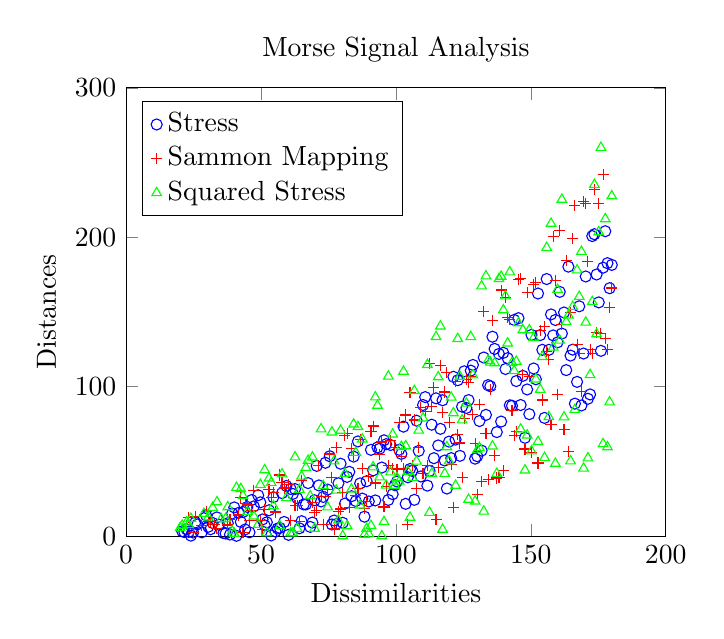
\begin{tikzpicture}
        \begin{axis}[
        only marks,                    % no lines
        xmin=0, xmax=200,              % x-axis limits
        ymin=0, ymax=300,              % y-axis limits
        xlabel={Dissimilarities},      % x-axis label
        ylabel={Distances},            % y-axis label
        title={Morse Signal Analysis}, % plot title
        legend pos=north west,         % legend position on plot
        legend cell align=left,        % text alignment within legend
        domain=20:180,                 % domain for plotted functions (not needed for scatter data)
        samples=200,                   % plot 200 samples
        ]
        \addplot[mark=o,blue] {x^2/200 + rand*x/3}; % add the first plot
        \addlegendentry{Stress}; % add the first plot's legend entry
        \addplot[mark=+,red]  {x^2/200 + rand*x/2}; % ...
        \addlegendentry{Sammon Mapping};
        \addplot[mark=triangle,green] {x^2/200 + rand*x/1.5};
        \addlegendentry{Squared Stress};
        \end{axis}
        \end{tikzpicture}
        
        \bigskip
        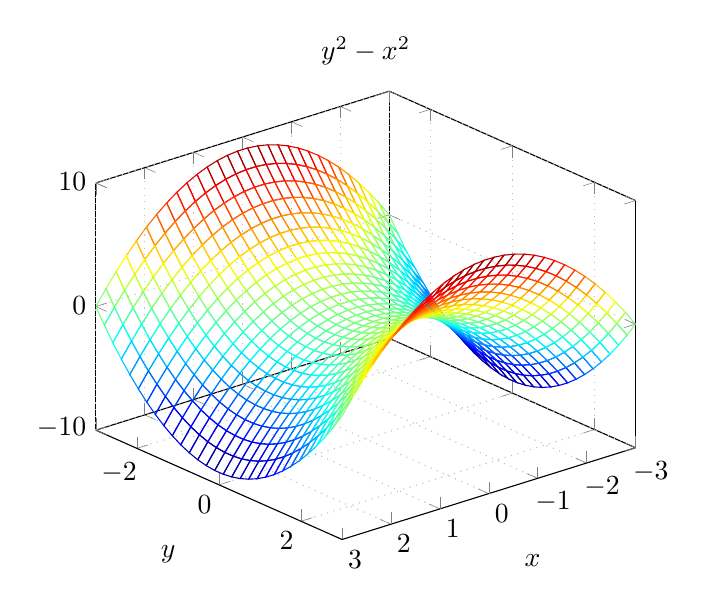
\begin{tikzpicture}
        \begin{axis}[
        grid=major,              % draw major gridlines
        major grid style=dotted, % dotted grid lines
        colormap/jet,            % colormap from MATLAB
        samples=30,              % 30 samples in each direction
        view={140}{30},          % configure plot view
        domain=-3:3,             % x varies from -3 to 3
        y domain=-3:3,           % y varies from -3 to 3
        zmin=-10, zmax=10,       % z-axis limits
        xlabel={$x$},            % x-axis label
        xtick={-3,-2,...,3},     % integer-spaced tick marks on the x-axis
        ylabel={$y$},            % y-axis label
        title={$y^2 - x^2$},     % plot title
        ]
        \addplot3[mesh] {y^2-x^2}; % make the mesh plot
        \end{axis}
        \end{tikzpicture}
\end{document}

%%% Local Variables:
%%% mode: latex
%%% TeX-master: t
%%% End:
